\chapter{Objective 4}

\section{Introduction}

Our heroes were heading towards the elevator. As they were passing through the Great Room, Grinch saw a splunk screen.
As he tried to log in, {\color{codegreen}Angel Candysalt} came rushing in the room. It turns out that Splunk is charging \footnote{I like Splunk, I'm just highlighting the subtle art of "The more sources the merrier, we may not need them and my rules may make no sense but I don't man that chair so I'm ok, merging my rules in production, kbye now.".} tons of money so only Santa and some elves are allowed to touch it.
The others were caught adding in random sources without properly QAing them. Not only the bill skyrocketed, we were buried with alerts.

Our two heroes started feeling like Santa had betrayed them but they continued with the elevator.
\subsection{A small bypass}
\textit{Narrator steps in again} If you inspect closely the data sent by the https://elevator.kringlecastle.com you will see that some data is passed in in the URL.
Up to this point, there is another nut that I haven't mentioned located near the Javascript machine. Using Chrome's tools, you can actually "get" all items available.

\begin{figure}[h!]
  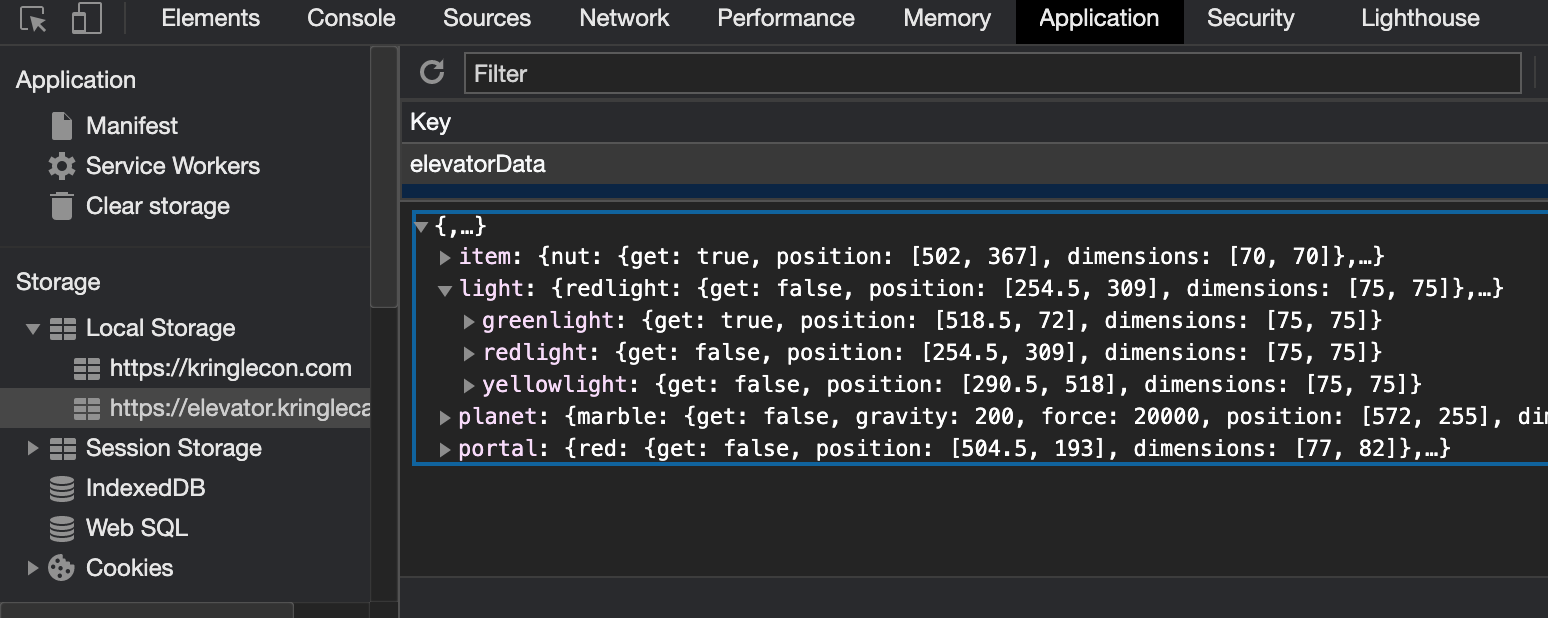
\includegraphics[scale=0.5]{chrome-data}
  \caption{Printscreen showcasing the data stored in the browser.}
\end{figure}

Altering the object is easy, you can directly add whatever objects/attributes you want in the URL, as evidenced in the following printscreen.
\newpage
\begin{figure}[h!]
  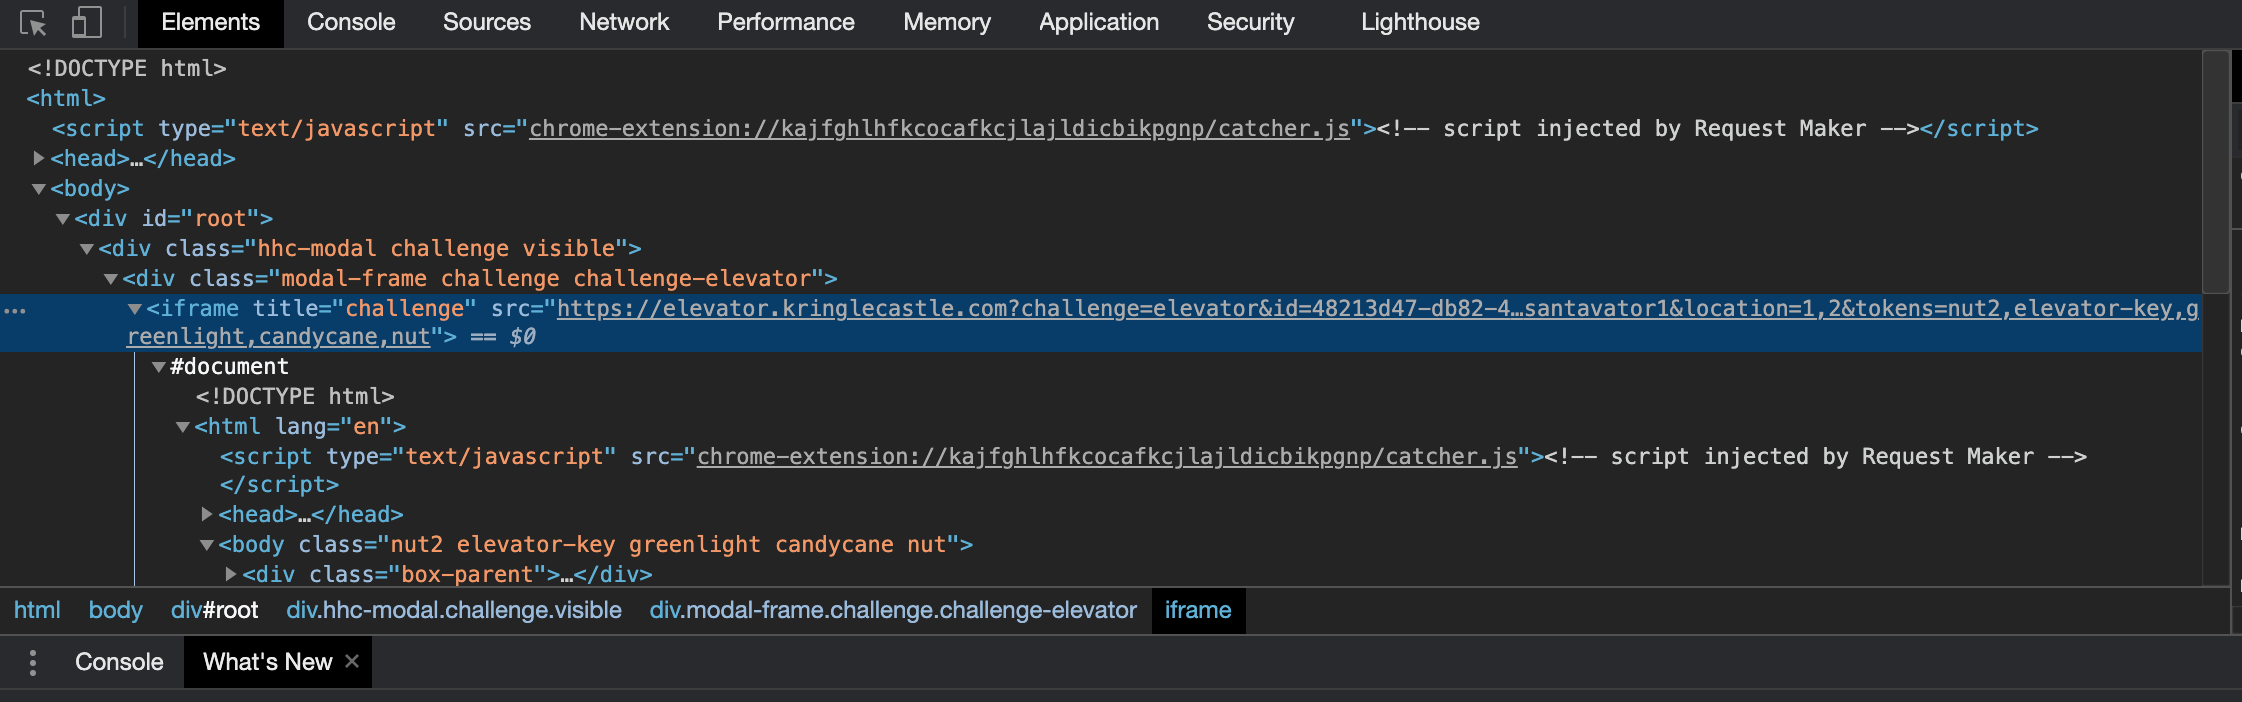
\includegraphics[scale=0.5]{chrome-url}
  \caption{The tokens= part of the URL can be changed to add any object.}
\end{figure}

- Go home narrator, this is our story.

\subsection {Back on track}
Cindy Lou quickly found a way to operate the Santavator.
\begin{figure}[h!]
  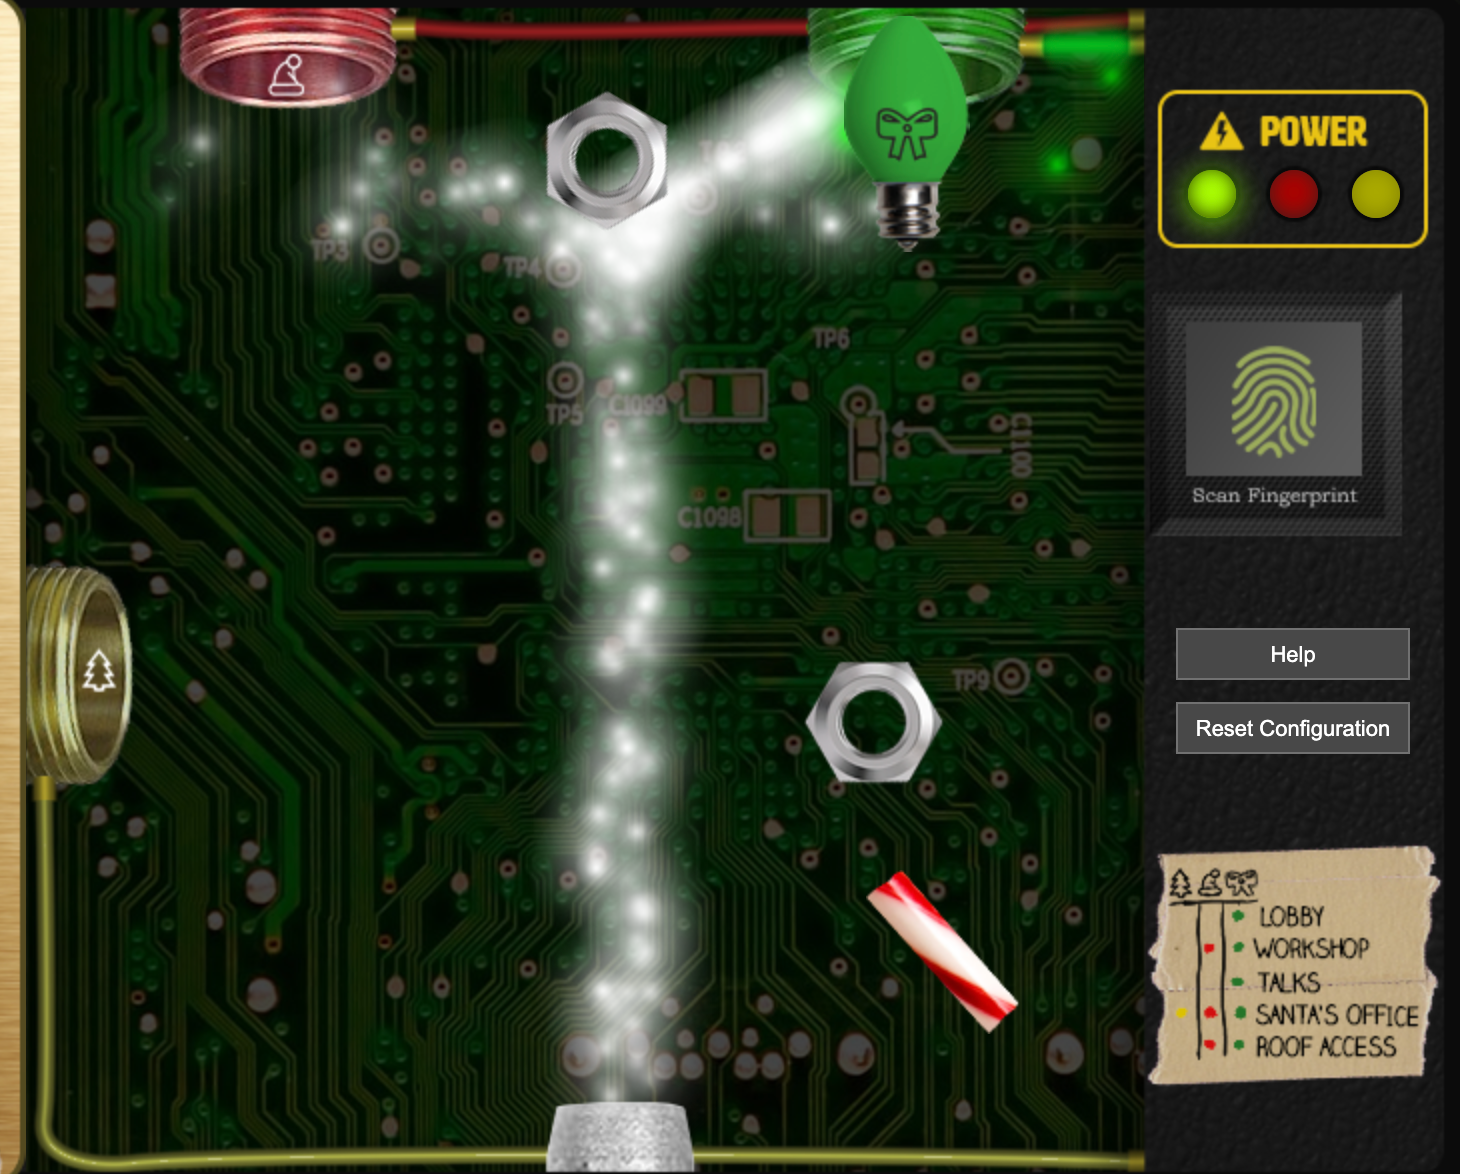
\includegraphics[scale=0.4]{Santavator-1}
  \caption{Power is headed to the Green bulb}
\end{figure}

Our heroes managed to operate the Santavator and head to the talks lobby.
